\chapter{Lecture 22 - Numerical Quadrature with MATLAB Built-in Functions}
\label{ch:lec22n}
\section{Objectives}
The objectives of this lecture are to:
\begin{itemize}
\item Describe and demonstrate the use of \lstinline[style=myMatlab]{trapz}.
\item Describe and demonstrate the use of \lstinline[style=myMatlab]{integral}, \lstinline[style=myMatlab]{integral2}, and \lstinline[style=myMatlab]{integral3}.
\end{itemize}
\setcounter{lstannotation}{0}

If you are doing your computing in a MATLAB environment, it makes sense to use MATLAB built-in functions for essentially all applications.  In this lecture we will explore the essential quadrature tools available in MATLAB.

\section{Integration with TRAPZ}
This is the function to use when you must integrate a function from sampled data.  Consider the example below.

\begin{marginfigure}
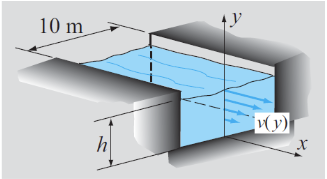
\includegraphics{lec22n-ex1.png}
\caption{Example water channel dimensions.}
\label{fig:lec22n-ex1}
\end{marginfigure}

\vspace{0.25cm}

\noindent\textbf{Example:} The flow rate $Q$, $\text{m}^3/\text{s}$, in the channel shown in Figure \ref{fig:lec22n-ex1} can be calculated by:

\begin{equation*}
Q = \int_{0}^{b} \ v(y) \ dy
\end{equation*}
where $v(y)$ is the water speed in $\text{m}/\text{s}$ and $h=5$ is the overall height of the water.  The water speed at different heights are given in Table \ref{tab:lec22n-ex1}.
\begin{margintable}
\begin{tabular}{|c|c|c|c|c|c|}
\hline
$y$ [m] & 0 & 0.3 & 0.5 & 1.0 & 1.5 \\ \hline
$x$ [m/s] & 0 & 0.4 & 0.5 & 0.56 & 0.6 \\ \hline
$y$ [m] & 2 & 2.5 & 3 & 4 & 5 \\ \hline
$x$ [m/s] & 0.63 & 0.66 & 0.68 & 0.71 & 0.74 \\ \hline
\end{tabular}
\caption{Water speed data taken at various channel depths.}
\label{tab:lec22n-ex1}
\end{margintable}

\noindent MATLAB's primary tool for numeric integration in cases like this is \lstinline[style=myMatlab]{trapz} which, as the name makes plain, is based on the trapezoidal rule.  The call syntax is:
\begin{enumerate}
\item \lstinline[style=myMatlab]{Q = trapz(Y)}.  This form assumes that the data provided in \lstinline[style=myMatlab]{Y} is uniformly spaced with unit interval between data points.  
\item \lstinline[style=myMatlab]{Q = trapz(X,Y)}.  With this syntax the user supplies the location of the data points.  They can non-uniformly spaced with any interval.  This is, of course, the form that we should use for this example problem.

\item \lstinline[style=myMatlab]{Q = trapz(X,Y,dim)}. This form allows for integrals in multiple dimensions.  Readers are encouraged to consult the MATLAB documentation for more details.  
\end{enumerate}

A straight-forward MATLAB implementation is provided in the listing below.
\begin{lstlisting}[style=myMatlab,name=lec22n-ex1]
clear
clc
close 'all'

y = [0 0.3 0.5 1 1.5 ...
    2 2.5 3 4 5]; % m, depth
v = [0 0.4 0.5 0.56 0.6 ...
    0.63 0.66 0.68 0.71 0.74];% m/s, speed

h = 10; % m, width of channel.

Q = h*trapz(y,v); % m^3/s, volumetric flow rate
fprintf('Q = %g m^3/s \n',Q);
\end{lstlisting}

\section{Integration with INTEGRAL}
The MATLAB function \lstinline[style=myMatlab]{integral} should be used for numeric integration in one dimension. This function uses adaptive integration over intervals with Gauss quadrature.\cite{shampine2008vectorized}  Interested readers are encouraged to locate and read the MATLAB file in which this built-in function is implemented.\sidenote{As of release 2023b, the function is implemented in MATLAB code and thus the details, in principle, are accessible to users.} As with other numeric integration algorithms the integral must be carried out over definite bounds but \emph{improper} integrals can be handled automatically.\sidenote{\textbf{Reminder:} an integral is said to be improper when either or both limits of integration are infinite or when the integrand diverges to infinity at one or more points in the range of integration.}

\vspace{0.2cm}

\noindent\textbf{Example:} Evaluate the the following integral using MATLAB's built-in function \lstinline[style=myMatlab]{integral}.
\begin{equation*}
I = \int_{0}^{\pi} \ \sin^{2}x \ dx
\end{equation*}
The basic call syntax is shown in the listing below.
\begin{lstlisting}[style=myMatlab,name=lec22n-ex2]
clear
clc
close 'all'

f = @(x) sin(x).^2;
a = 0; b = pi;
int_f = integral(f,a,b);
fprintf('I = %g \n',int_f);
\end{lstlisting}

As with many of MATLAB's built-in function, a user can further control behavior of the function by specifying name/value pairs for optional arguments, \lstinline[style=myMatlab]{I = integral(fun,a,b,Name,Value)}. Two important name/value pairs are:
\begin{enumerate}
\item \lstinline[style=myMatlab]{'RelTol'}. The corresponding argument should be a non-negative real number; the default value is $10^{-6}$.  The algorithm estimates the relative error of the computed integral---$|q - Q|/|Q|$, where $q$ is the computed result and $Q$ is the (unknown) exact value.  

\item \lstinline[style=myMatlab]{'AbsTol'}.  The corresponding argument should be a non-negative real number; the default value is $10^{-10}$.
\end{enumerate}
Note that MATLAB uses both the absolute and relative error tolerance as stopping criteria in the \lstinline[style=myMatlab]{integral} implementation.  You should generally specify both absolute and relative tolerances if is important that you obtain greater precision in your results.

\section{Multiple Integrals}
In this course we will not go through the details of multi-dimensional numeric integration.  MATLAB provides facilitates integration in 2- or 3-dimensions with the built-in functions \lstinline[style=myMatlab]{integral2} and \lstinline[style=myMatlab]{integral3}.\sidenote{Evidently there are no points for creativity in function naming at MathWorks.}  

\vspace{0.25cm}

\noindent\textbf{Example:} Evaluate the integral:

\begin{equation*}
\int_{-\infty}^{\infty} \int_{-\infty}^{\infty} \int_{-\infty}^{\infty} \sqrt{x^2 + y^2 + z^2}e^{-\left(x^2 + y^2 + z^2\right)} \ \text{dx dy dz}
\end{equation*}

Using \lstinline[style=myMatlab]{integral3}:
\begin{lstlisting}[style=myMatlab,name=lec22n-ex3]
clear
clc
close 'all'

fun = @(x,y,z) sqrt(x.^2+y.^2+z.^2).*exp(-(x.^2+y.^2+z.^2));
I = integral3(fun,-inf,inf,-inf,inf,-inf,inf);

I_exact = 2*pi;

I_rel_error = abs(I - I_exact)/abs(I_exact);
fprintf('I = %g \n',I);
fprintf('relative error: %g \n',I_rel_error);
\end{lstlisting}

\noindent It cannot be discerned by this example, but the last six arguments comprise the lower and upper bounds of integration in each dimension---lower and upper bounds in the first dimension, followed by the lower and upper bounds in the second dimension, then the lower and upper bounds in the third dimension.  The ordering of dimensions---e.g., in this case, $x$, $y$, and $z$---are the same as the ordering of arguments in the function used for the integrand.  

One important detail to remember is that, for integration in polar, cylindrical, or spherical coordinates, the differential volume element is \emph{not} included.  This is illustrated in the example below.

\vspace{0.25cm}

\noindent\textbf{Example:} Under the assumptions of single-group diffusion theory, the flux, $\phi(r,z)$, in a homogeneous, bare, cylindrical (nuclear) reactor of radius $R$ and height $H$ is given by:

\begin{equation*}
\phi(r,z) = C J_0\left(\frac{2.405r}{R} \right)\cos{\left(\frac{\pi z}{H} \right)}
\end{equation*} 
Where $J_{0}$ is the Bessel function of the first kind of order zero and $C$ is a constant. One parameter of interest is the ratio of the peak to average flux in the reactor.  The average flux is:\marginnote{

\vspace{1.5cm}

\noindent Note the extra factor of $r$ for the differential volume element: $r d\theta dr dz$.  

}
\begin{align*}
\phi_{\text{avg}} &= \frac{\int \phi \ dV}{V} \\
&= \frac{\int_{-\sfrac{H}{2}}^{\sfrac{H}{2}} \int_{0}^{R}  \int_{0}^{2 \pi} \phi(r,z) \ r d\theta drdz }{\pi R^2 H} \\
&= \frac{2 \pi  \int_{-\sfrac{H}{2}}^{\sfrac{H}{2}} \int_{0}^{R} \phi(r,z) \ rdrdz }{\pi R^2 H}
\end{align*}
and the peak flux $\phi_{\text{peak}}$ is equal to $C$.  With this information, we can use MATLAB to calculate the ratio of peak to average flux:
\marginnote{

\vspace{3.0cm}

\ref{lst:ann22n-1} Here the extra factor of $r$ is for the differential volume.  Hopefully it is clear that MATLAB does not do this automatically; it is incumbent upon the user to include details like this. 

}
\begin{lstlisting}[style=myMatlab,name=lec22n-ex4]
clear
clc
close 'all'

R = 3; H = 6;
C = 1;
P = @(r,z) C*besselj(0,2.405*r/R).*cos(pi*z/H);

totP = 2*pi*integral2(@(r,z) P(r,z).*r,0,R,-H/2,H/2); /*!\annotation{lst:ann22n-1}!*/
V = pi*(R.^2)*H;
AvgP = totP/V;
fprintf('Peak/Avg power = %g \n',C./AvgP);
\end{lstlisting}
The output of this script is approximately 3.6387 which is a standard result in reactor physics based on diffusion theory.


